\documentclass[11pt,a4paper]{article}
\usepackage[utf8]{inputenc}
\usepackage[T1]{fontenc}
\usepackage{lmodern}
\usepackage{geometry}
\usepackage{hyperref}
\usepackage{listings}
\usepackage{xcolor}
\usepackage{booktabs}
\usepackage{array}
\usepackage{fancyhdr}
\usepackage{enumitem}
\usepackage{float}
\usepackage{mdframed}
\usepackage{tikz}
\usepackage{graphicx}
\usetikzlibrary{shapes,arrows,positioning,fit,backgrounds,calc}

\geometry{margin=1in}

\definecolor{hydra-blue}{RGB}{5,32,73}
\definecolor{code-bg}{RGB}{248,248,248}
\definecolor{warning-bg}{RGB}{255,243,205}
\definecolor{success-bg}{RGB}{212,237,218}
\definecolor{info-bg}{RGB}{217,237,247}
\definecolor{gpu-green}{RGB}{118,185,0}
\definecolor{cerberus-orange}{RGB}{255,152,0}
\definecolor{chimera-purple}{RGB}{156,39,176}

\hypersetup{colorlinks=true,linkcolor=hydra-blue,urlcolor=blue}

\lstdefinestyle{bash}{backgroundcolor=\color{code-bg},basicstyle=\ttfamily\small,breaklines=true,frame=single,numbers=none}
\lstdefinestyle{js}{backgroundcolor=\color{code-bg},basicstyle=\ttfamily\small,breaklines=true,frame=single,numbers=left,language=Java}

\newmdenv[backgroundcolor=warning-bg,linewidth=0pt,innerleftmargin=10pt,innerrightmargin=10pt,innertopmargin=10pt,innerbottommargin=10pt]{warningbox}
\newmdenv[backgroundcolor=success-bg,linewidth=0pt,innerleftmargin=10pt,innerrightmargin=10pt,innertopmargin=10pt,innerbottommargin=10pt]{successbox}
\newmdenv[backgroundcolor=info-bg,linewidth=0pt,innerleftmargin=10pt,innerrightmargin=10pt,innertopmargin=10pt,innerbottommargin=10pt]{infobox}

\pagestyle{fancy}
\fancyhf{}
\fancyhead[L]{\textbf{Hydra Infrastructure}}
\fancyhead[R]{\textbf{Management Guide}}
\fancyfoot[C]{\thepage}
\setlength{\headheight}{14pt}

\title{\textbf{Hydra Infrastructure Management Guide}\\[0.5em]\large Student Container Platform Administration}
\author{Computer Science Department\\SUNY New Paltz}
\date{Last Updated: January 2025}

\begin{document}
\maketitle
\tableofcontents
\newpage

\section{System Overview}

Hydra is a containerized development platform providing persistent development environments for Computer Science students and faculty at SUNY New Paltz. The system uses SAML 2.0 Single Sign-On via Azure AD and Docker for container orchestration across a 3-node cluster.

\subsection{Key Features}
\begin{itemize}
    \item \textbf{SSO Authentication:} Azure AD SAML 2.0 with automatic user provisioning
    \item \textbf{Persistent Containers:} One development environment per student with data persistence
    \item \textbf{Built-in Services:} VS Code (code-server), Jupyter Notebook, Docker-in-Docker
    \item \textbf{SSH Access:} Direct SSH access to containers via assigned ports
    \item \textbf{GPU Computing:} Access to NVIDIA GPUs on Chimera and Cerberus nodes
    \item \textbf{Dynamic Routing:} Traefik-based routing for custom web applications
    \item \textbf{Resource Management:} Time-limited resource allocations with automatic expiry
    \item \textbf{Integration:} OpenWebUI (GPT) and n8n account management
\end{itemize}

\subsection{Access URLs}
\begin{table}[H]
\centering
\begin{tabular}{lll}
\toprule
\textbf{Service} & \textbf{URL} & \textbf{Description} \\
\midrule
Dashboard & \texttt{https://hydra.newpaltz.edu/dashboard} & Main user interface \\
OpenWebUI & \texttt{https://gpt.hydra.newpaltz.edu/} & AI chat interface \\
VS Code & \texttt{https://hydra.newpaltz.edu/students/\{user\}/vscode} & Browser IDE \\
Jupyter & \texttt{https://hydra.newpaltz.edu/students/\{user\}/jupyter} & Notebooks \\
Servers & \texttt{https://hydra.newpaltz.edu/servers} & Cluster status \\
\bottomrule
\end{tabular}
\end{table}

\section{Cluster Architecture}

The Hydra platform operates across a 3-node cluster, each with specialized roles.

\subsection{Cluster Nodes}

\begin{table}[H]
\centering
\begin{tabular}{llllp{4cm}}
\toprule
\textbf{Node} & \textbf{IP} & \textbf{Role} & \textbf{GPU} & \textbf{Description} \\
\midrule
Hydra & 192.168.1.160 & Control Plane & None & Main server, ZFS storage, student containers \\
Chimera & 192.168.1.150 & Inference & 3x RTX 3090 & OpenWebUI, inference workloads \\
Cerberus & 192.168.1.242 & Training & 2x RTX 5090 & Student GPU training \\
\bottomrule
\end{tabular}
\end{table}

\subsection{Architecture Diagram}

\begin{center}
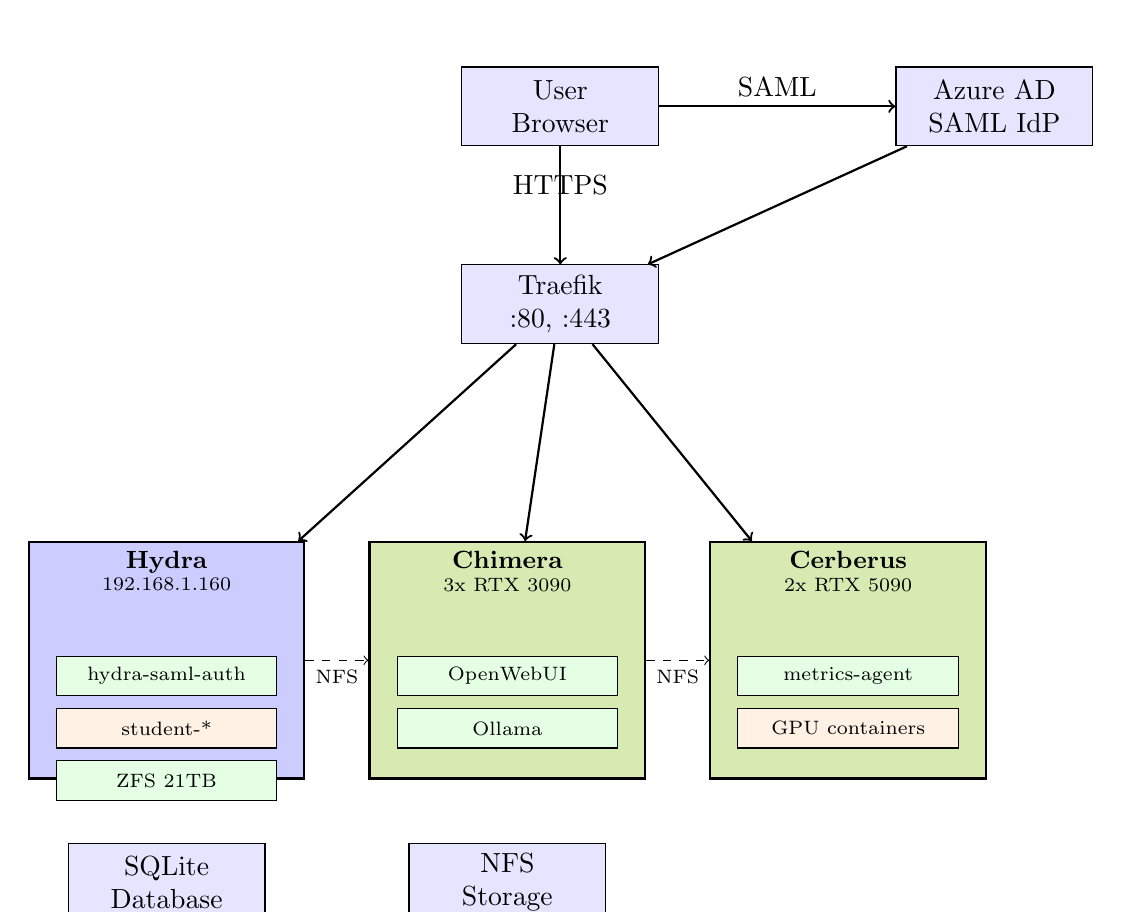
\begin{tikzpicture}[
    node distance=1.2cm,
    box/.style={rectangle, draw, fill=blue!10, minimum width=2.5cm, minimum height=1cm, align=center},
    server/.style={rectangle, draw, thick, fill=blue!20, minimum width=3.5cm, minimum height=3cm, align=center},
    gpu/.style={rectangle, draw, thick, fill=gpu-green!30, minimum width=3.5cm, minimum height=3cm, align=center},
    service/.style={rectangle, draw, fill=green!10, minimum width=2.8cm, minimum height=0.5cm, align=center, font=\scriptsize},
    container/.style={rectangle, draw, fill=orange!10, minimum width=2.8cm, minimum height=0.5cm, align=center, font=\scriptsize},
    arrow/.style={->, thick},
    dashed_arrow/.style={->, dashed}
]

% External
\node[box] (user) {User\\Browser};
\node[box, right=3cm of user] (azure) {Azure AD\\SAML IdP};

% Traefik
\node[box, below=1.5cm of user] (traefik) {Traefik\\:80, :443};

% Hydra Server - position with explicit coordinates
\node[server, below=2.5cm of traefik, xshift=-5cm] (hydra) {};
\node[font=\small\bfseries, anchor=north] at (hydra.north) {Hydra};
\node[font=\scriptsize, anchor=north] at ([yshift=-0.35cm]hydra.north) {192.168.1.160};
\node[service] at ([yshift=-0.2cm]hydra.center) (hydra-app) {hydra-saml-auth};
\node[container, below=0.15cm of hydra-app] (student1) {student-*};
\node[service, below=0.15cm of student1] (zfs) {ZFS 21TB};

% Chimera Server
\node[gpu, right=0.8cm of hydra] (chimera) {};
\node[font=\small\bfseries, anchor=north] at (chimera.north) {Chimera};
\node[font=\scriptsize, anchor=north] at ([yshift=-0.35cm]chimera.north) {3x RTX 3090};
\node[service] at ([yshift=-0.2cm]chimera.center) (openwebui) {OpenWebUI};
\node[service, below=0.15cm of openwebui] (ollama) {Ollama};

% Cerberus Server
\node[gpu, right=0.8cm of chimera] (cerberus) {};
\node[font=\small\bfseries, anchor=north] at (cerberus.north) {Cerberus};
\node[font=\scriptsize, anchor=north] at ([yshift=-0.35cm]cerberus.north) {2x RTX 5090};
\node[service] at ([yshift=-0.2cm]cerberus.center) (metrics) {metrics-agent};
\node[container, below=0.15cm of metrics] (gpu-student) {GPU containers};

% Storage
\node[box, below=0.8cm of hydra] (db) {SQLite\\Database};
\node[box, below=0.8cm of chimera] (nfs) {NFS\\Storage};

% Arrows
\draw[arrow] (user) -- node[above] {HTTPS} (traefik);
\draw[arrow, bend left=20] (user) -- node[above] {SAML} (azure);
\draw[arrow, bend left=20] (azure) -- (traefik);
\draw[arrow] (traefik) -- (hydra);
\draw[arrow] (traefik) -- (chimera);
\draw[arrow] (traefik) -- (cerberus);
\draw[dashed_arrow] (hydra) -- node[below, font=\scriptsize] {NFS} (chimera);
\draw[dashed_arrow] (chimera) -- node[below, font=\scriptsize] {NFS} (cerberus);

\end{tikzpicture}
\end{center}

\subsection{Storage Configuration}

\begin{table}[H]
\centering
\begin{tabular}{llll}
\toprule
\textbf{Node} & \textbf{Storage} & \textbf{Capacity} & \textbf{Purpose} \\
\midrule
Hydra & ZFS RAID-10 & 21 TB & Student volumes, primary data \\
Hydra & Seagate SSD & 1.1 TB & Daily backups \\
Chimera & NFS mount & -- & Student data access \\
Cerberus & NFS mount & -- & Student data access \\
\bottomrule
\end{tabular}
\end{table}

\subsection{Component Overview}

\begin{table}[H]
\centering
\begin{tabular}{llp{6cm}}
\toprule
\textbf{Component} & \textbf{Port} & \textbf{Description} \\
\midrule
Traefik & 80, 443 & Reverse proxy, TLS termination, routing \\
hydra-saml-auth & 6969 & SAML auth, dashboard, container management \\
OpenWebUI & 3000 & AI chat interface (Ollama frontend) \\
Ollama & 11434 & LLM inference engine \\
metrics-agent & 9100 & Node metrics collection (GPU nodes) \\
Student Containers & Dynamic & Per-user development environments \\
\bottomrule
\end{tabular}
\end{table}

\subsection{Network Architecture}

Student containers operate on an isolated Docker network (\texttt{hydra\_students\_net}) with:
\begin{itemize}
    \item No direct internet access (configurable)
    \item Internal DNS resolution
    \item Traefik-mediated external access via ForwardAuth
    \item Cross-node NFS access for GPU workloads
\end{itemize}

\section{Authentication System}

\subsection{SAML 2.0 SSO Flow}

\begin{center}
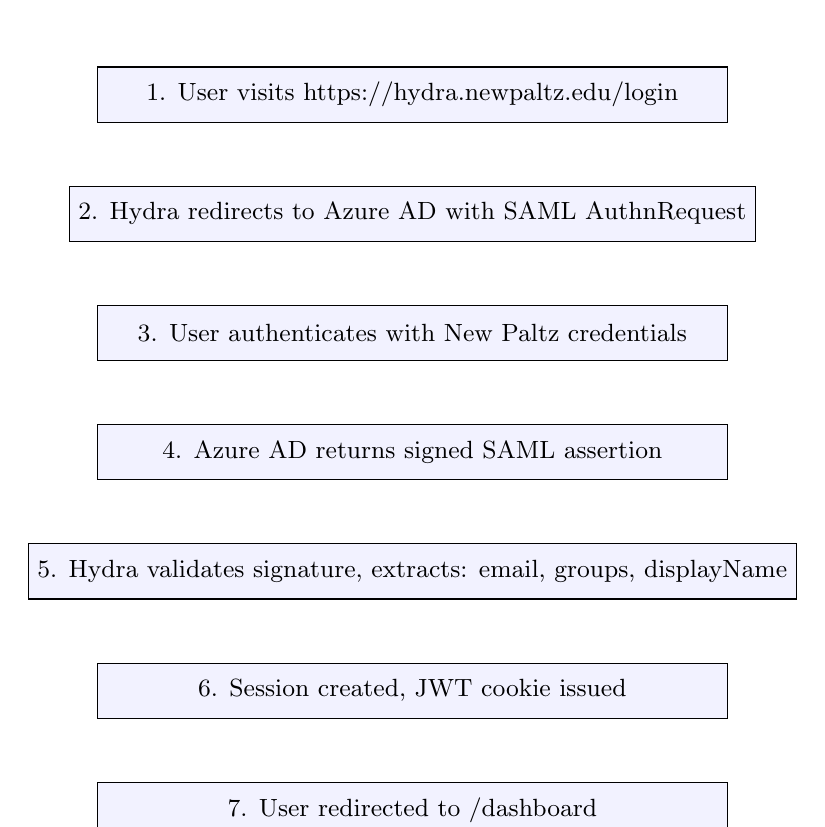
\begin{tikzpicture}[
    node distance=0.8cm,
    stepbox/.style={rectangle, draw, fill=blue!5, minimum width=8cm, minimum height=0.7cm, align=left, font=\small}
]
\node[stepbox] (s1) {1. User visits https://hydra.newpaltz.edu/login};
\node[stepbox, below=of s1] (s2) {2. Hydra redirects to Azure AD with SAML AuthnRequest};
\node[stepbox, below=of s2] (s3) {3. User authenticates with New Paltz credentials};
\node[stepbox, below=of s3] (s4) {4. Azure AD returns signed SAML assertion};
\node[stepbox, below=of s4] (s5) {5. Hydra validates signature, extracts: email, groups, displayName};
\node[stepbox, below=of s5] (s6) {6. Session created, JWT cookie issued};
\node[stepbox, below=of s6] (s7) {7. User redirected to /dashboard};
\end{tikzpicture}
\end{center}

\subsection{Session Management}

Sessions are managed via:
\begin{itemize}
    \item \textbf{Express Session:} Server-side session storage in SQLite
    \item \textbf{JWT Cookie:} Site-wide authentication cookie for cross-service SSO
    \item \textbf{JWKS Endpoint:} Public key endpoint for JWT verification by other services
\end{itemize}

\begin{infobox}
\textbf{JWT Configuration:}
\begin{itemize}
    \item TTL: Configurable via \texttt{JWT\_TTL\_SECONDS} (default: 86400)
    \item Algorithm: RS256
    \item Cookie Domain: \texttt{.newpaltz.edu}
\end{itemize}
\end{infobox}

\section{Container System}

\subsection{Student Container Features}

Each student receives a single persistent container with:

\begin{table}[H]
\centering
\begin{tabular}{lp{8cm}}
\toprule
\textbf{Feature} & \textbf{Details} \\
\midrule
Node.js & Latest LTS via nvm \\
Python & 3.11+ with pip, venv, Jupyter \\
Java & OpenJDK 21 \\
Docker & Full Docker-in-Docker support (privileged mode) \\
VS Code & code-server browser IDE with extensions \\
Jupyter & Notebook and JupyterLab \\
SSH & Direct SSH access via assigned port \\
Tools & Git, curl, wget, build-essential, etc. \\
\bottomrule
\end{tabular}
\end{table}

\subsection{SSH Access}

Students can access their containers via SSH from any terminal:

\begin{lstlisting}[style=bash]
# Connect to your container
ssh -p <assigned_port> student@hydra.newpaltz.edu

# Example with port 2222
ssh -p 2222 student@hydra.newpaltz.edu
\end{lstlisting}

\begin{itemize}
    \item SSH ports are dynamically assigned from range 2200-2299
    \item Password is displayed in the dashboard after container creation
    \item SSH supports key-based authentication (add keys to \texttt{\~{}/.ssh/authorized\_keys})
\end{itemize}

\begin{infobox}
\textbf{SSH Setup:} Each container runs an SSH server via supervisord. The SSH port and password are shown in the dashboard under "SSH Access" section.
\end{infobox}

\subsection{Resource Presets}

\begin{table}[H]
\centering
\begin{tabular}{llllll}
\toprule
\textbf{Preset} & \textbf{RAM} & \textbf{CPU} & \textbf{Storage} & \textbf{GPU} & \textbf{Approval} \\
\midrule
Minimal & 256 MB & 0.5 & 5 GB & 0 & Auto \\
Conservative & 512 MB & 1 & 10 GB & 0 & Auto \\
Standard & 1 GB & 1 & 20 GB & 0 & Auto \\
Enhanced & 2 GB & 2 & 40 GB & 0 & Required \\
GPU Inference & 32 GB & 8 & 100 GB & 1 & Required \\
GPU Training & 48 GB & 16 & 200 GB & 2 & Required \\
\bottomrule
\end{tabular}
\end{table}

\begin{warningbox}
\textbf{GPU Access:} GPU presets run on Chimera (inference) or Cerberus (training). Chimera GPUs are shared with OpenWebUI; use Cerberus for dedicated GPU work.
\end{warningbox}

\section{Resource Management}

\subsection{Time-Limited Allocations}

Resource allocations are time-limited to ensure fair sharing among students:

\begin{table}[H]
\centering
\begin{tabular}{lll}
\toprule
\textbf{Duration} & \textbf{Approval} & \textbf{Use Case} \\
\midrule
1 Day (Default) & Auto & Quick testing \\
3 Days & Auto & Short assignment \\
1 Week & Auto & Short projects \\
2 Weeks & Auto & Standard projects \\
1 Month & Auto & Semester project \\
2 Months & Required & Extended project \\
3 Months & Required & Full semester \\
\bottomrule
\end{tabular}
\end{table}

\subsection{Resource Expiry}

When a resource allocation expires:
\begin{enumerate}
    \item Configuration resets to \textbf{minimal} preset
    \item Container moves back to \textbf{Hydra} node
    \item Container automatically \textbf{restarts} to apply new limits
    \item Student receives notification (if email configured)
\end{enumerate}

The expiry checker runs hourly via the \texttt{resource-expiry} service.

\subsection{Requesting Additional Resources}

\begin{enumerate}
    \item Navigate to Dashboard $\rightarrow$ Configure Resources
    \item Select desired preset, node, and duration
    \item Submit request (auto-approved if within thresholds)
    \item If approval required, admin reviews within 7 days
\end{enumerate}

\begin{infobox}
\textbf{Auto-Approval Thresholds (Hydra only):}
\begin{itemize}
    \item Memory: up to 2 GB
    \item CPU: up to 2 cores
    \item Storage: up to 20 GB
\end{itemize}
\end{infobox}

\section{GPU Computing}

\subsection{GPU Node Configuration}

\begin{table}[H]
\centering
\begin{tabular}{lllll}
\toprule
\textbf{Node} & \textbf{GPUs} & \textbf{Model} & \textbf{VRAM} & \textbf{Primary Use} \\
\midrule
Chimera & 3 & RTX 3090 & 72 GB total & OpenWebUI/Inference \\
Cerberus & 2 & RTX 5090 & 64 GB total & Student training \\
\bottomrule
\end{tabular}
\end{table}

\subsection{GPU Access Guidelines}

\begin{itemize}
    \item \textbf{Cerberus (Recommended):} Use for GPU training and student projects. RTX 5090 offers newer architecture with 32GB VRAM per card.
    \item \textbf{Chimera:} Reserved for OpenWebUI inference. 1 GPU is reserved for Ollama. Only use if Cerberus is unavailable.
\end{itemize}

\subsection{Requesting GPU Access}

\begin{enumerate}
    \item Select "GPU Training" preset in Configure Resources
    \item Choose Cerberus as target node
    \item Provide justification for GPU access
    \item Wait for admin approval
\end{enumerate}

\section{Backup System}

\subsection{Daily Cluster Backups}

All cluster nodes are backed up daily at 1:00 AM to the Seagate drive on Hydra.

\begin{table}[H]
\centering
\begin{tabular}{ll}
\toprule
\textbf{Setting} & \textbf{Value} \\
\midrule
Backup Location & \texttt{/mnt/sdh4/backups/} \\
Schedule & Daily at 1:00 AM \\
Method & rsync with compression \\
Log File & \texttt{/var/log/cluster-backup.log} \\
\bottomrule
\end{tabular}
\end{table}

\subsection{What Gets Backed Up}

\begin{itemize}
    \item \textbf{Hydra:} Full OS, configuration, application code (excludes Docker volumes)
    \item \textbf{Chimera:} Full OS, NVIDIA drivers, OpenWebUI config
    \item \textbf{Cerberus:} Full OS, NVIDIA drivers, metrics agent
\end{itemize}

\subsection{Backup Exclusions}

The following are excluded from backups:
\begin{itemize}
    \item \texttt{/dev/*}, \texttt{/proc/*}, \texttt{/sys/*}, \texttt{/run/*}
    \item \texttt{/tmp/*}, \texttt{/var/tmp/*}, \texttt{/var/cache/*}
    \item \texttt{/mnt/*}, \texttt{/media/*}, \texttt{/lost+found}
    \item \texttt{/var/lib/docker/*} (Docker data)
\end{itemize}

\subsection{Manual Backup}

\begin{lstlisting}[style=bash]
# Run backup manually
sudo /home/infra/backup-cluster.sh

# Check backup status
cat /var/log/cluster-backup.log

# View backup sizes
du -sh /mnt/sdh4/backups/*
\end{lstlisting}

\section{File Structure}

\begin{lstlisting}[style=bash]
hydra-saml-auth/
|-- index.js              # Main entry: SAML, JWT/JWKS, routes, WebSocket
|-- routes/
|   |-- containers.js     # Container lifecycle, services, ports, logs
|   |-- resource-requests.js  # Resource allocation requests
|   |-- webui-api.js      # OpenWebUI account proxy
|   |-- n8n-api.js        # n8n account management
|   |-- servers-api.js    # Cluster status endpoints
|   |-- admin.js          # Admin panel routes
|-- services/
|   |-- db-init.js        # Database initialization and migrations
|   |-- resource-expiry.js    # Time-limited resource expiry checker
|   |-- activity-logger.js    # Activity tracking
|   |-- email-notifications.js # Email alerts
|   |-- metrics-collector.js  # Node metrics collection
|-- config/
|   |-- resources.js      # Resource presets and node configuration
|-- agents/
|   |-- metrics-agent.js  # Node.js metrics agent (Hydra)
|-- scripts/
|   |-- metrics-agent.py  # Python metrics agent (GPU nodes)
|-- views/                # EJS templates
|-- student-container/
|   |-- Dockerfile        # Ubuntu 22.04 + dev tools + SSH
|   |-- supervisord.conf  # Process manager config (incl. sshd)
|   |-- entrypoint.sh     # Container startup
|-- ansible/              # Cluster deployment playbooks
|   |-- inventory.yml     # Node definitions
|   |-- playbooks/        # Deployment scripts
|-- docker-compose.yaml   # Production stack
|-- docs/                 # Documentation
\end{lstlisting}

\section{Common Operations}

\subsection{View Running Containers}
\begin{lstlisting}[style=bash]
docker ps --filter "name=student-"
\end{lstlisting}

\subsection{Access Container Shell}
\begin{lstlisting}[style=bash]
docker exec -it student-<username> /bin/bash
\end{lstlisting}

\subsection{View Container Logs}
\begin{lstlisting}[style=bash]
docker logs -f student-<username> --tail=100
\end{lstlisting}

\subsection{Restart a Container}
\begin{lstlisting}[style=bash]
docker restart student-<username>
\end{lstlisting}

\subsection{Remove a Stuck Container}
\begin{lstlisting}[style=bash]
docker rm -f student-<username>
\end{lstlisting}

\subsection{Rebuild Student Container Image}
\begin{lstlisting}[style=bash]
cd student-container
docker build -t hydra-student-container:latest .
\end{lstlisting}

\begin{infobox}
\textbf{Note:} Students with existing containers must recreate them to use updated images.
\end{infobox}

\subsection{Check Cluster Node Status}
\begin{lstlisting}[style=bash]
# Check metrics from Chimera
curl http://192.168.1.150:9100/metrics

# Check metrics from Cerberus
curl http://192.168.1.242:9100/metrics
\end{lstlisting}

\subsection{Trigger Resource Expiry Check}
\begin{lstlisting}[style=bash]
# From within the application
curl http://localhost:6969/api/admin/resource-expiry/check
\end{lstlisting}

\section{Service Management}

\subsection{Restart Main Service}
\begin{lstlisting}[style=bash]
docker compose restart hydra-saml-auth
\end{lstlisting}

\subsection{Rebuild and Redeploy}
\begin{lstlisting}[style=bash]
docker compose build hydra-saml-auth
docker compose up -d hydra-saml-auth
\end{lstlisting}

\subsection{View Service Logs}
\begin{lstlisting}[style=bash]
docker compose logs -f hydra-saml-auth
\end{lstlisting}

\subsection{Check Traefik Routing}
\begin{lstlisting}[style=bash]
docker compose logs traefik | grep -i error
curl -I https://hydra.newpaltz.edu/
\end{lstlisting}

\subsection{Manage Metrics Agent (GPU Nodes)}
\begin{lstlisting}[style=bash]
# On Chimera or Cerberus
sudo systemctl status metrics-agent
sudo systemctl restart metrics-agent
sudo journalctl -u metrics-agent -f
\end{lstlisting}

\section{Troubleshooting}

\subsection{Authentication Issues}

\begin{table}[H]
\centering
\begin{tabular}{lp{8cm}}
\toprule
\textbf{Symptom} & \textbf{Solution} \\
\midrule
SAML assertion invalid & Verify \texttt{METADATA\_URL} and \texttt{SAML\_SP\_ENTITY\_ID} match Azure config exactly \\
Cookie not set & Check \texttt{COOKIE\_DOMAIN}, ensure HTTPS, check browser settings \\
JWT verification fails & Verify JWKS endpoint accessible, check key rotation \\
\bottomrule
\end{tabular}
\end{table}

\subsection{Container Issues}

\begin{table}[H]
\centering
\begin{tabular}{lp{8cm}}
\toprule
\textbf{Symptom} & \textbf{Solution} \\
\midrule
Container won't initialize & Verify \texttt{hydra-student-container:latest} image exists \\
Container 404 & Check container is on \texttt{hydra\_students\_net}, Traefik running \\
Service won't start & Check supervisord logs inside container \\
Port routing fails & Verify port not reserved (8443, 8888) and not in use \\
SSH not working & Check sshd process in container, verify port assignment \\
\bottomrule
\end{tabular}
\end{table}

\subsection{GPU Issues}

\begin{table}[H]
\centering
\begin{tabular}{lp{8cm}}
\toprule
\textbf{Symptom} & \textbf{Solution} \\
\midrule
GPU not detected & Run \texttt{nvidia-smi} on host, check NVIDIA drivers \\
GPU container fails & Verify nvidia-container-toolkit installed \\
Metrics not showing & Check metrics-agent service, firewall port 9100 \\
\bottomrule
\end{tabular}
\end{table}

\subsection{Service-Specific Issues}

\begin{itemize}
    \item \textbf{VS Code not loading:} Check code-server process, ForwardAuth working
    \item \textbf{Jupyter issues:} Verify \texttt{NotebookApp.base\_url} setting
    \item \textbf{Docker-in-Docker fails:} Container must have privileged mode
    \item \textbf{Files not persisting:} Only \texttt{/home/student/} is persisted
    \item \textbf{Resource expiry not working:} Check resource-expiry service logs
\end{itemize}

\section{Ansible Deployment}

\subsection{Cluster Setup Overview}

The cluster can be deployed using Ansible playbooks in \texttt{ansible/} directory:

\begin{lstlisting}[style=bash]
# Full cluster deployment
cd ansible
ansible-playbook -i inventory.yml playbooks/site.yml
\end{lstlisting}

\subsection{Playbook Execution Order}

\begin{enumerate}
    \item \texttt{00-preflight-backup.yml} - Create backups before changes
    \item \texttt{01-prepare-nodes.yml} - Install packages, configure kernel
    \item \texttt{02-rke2-server.yml} - Setup RKE2 control plane
    \item \texttt{03-rke2-agents.yml} - Join GPU nodes to cluster
    \item \texttt{04-gpu-setup.yml} - Configure NVIDIA drivers and GPU Operator
    \item \texttt{05-deploy-hydra.yml} - Deploy Hydra application stack
\end{enumerate}

\subsection{Inventory Configuration}

The cluster inventory is defined in \texttt{ansible/inventory.yml}:

\begin{lstlisting}[style=bash]
# Key variables
rke2_version: "v1.28.4+rke2r1"
cluster_domain: hydra.newpaltz.edu
nfs_server: "192.168.1.160"
nfs_path: "/srv/hydra-nfs"
\end{lstlisting}

\section{Environment Configuration}

\subsection{Required Variables}
\begin{table}[H]
\centering
\begin{tabular}{lp{7cm}}
\toprule
\textbf{Variable} & \textbf{Description} \\
\midrule
\texttt{BASE\_URL} & External URL (https://hydra.newpaltz.edu) \\
\texttt{METADATA\_URL} & Azure AD federation metadata URL \\
\texttt{SAML\_SP\_ENTITY\_ID} & SP Entity ID (must match Azure exactly) \\
\texttt{COOKIE\_DOMAIN} & Cookie scope (.newpaltz.edu) \\
\texttt{PORT} & Service port (default: 6969) \\
\texttt{DB\_PATH} & Database path (/app/data/webui.db) \\
\bottomrule
\end{tabular}
\end{table}

\subsection{Optional Variables}
\begin{table}[H]
\centering
\begin{tabular}{lp{7cm}}
\toprule
\textbf{Variable} & \textbf{Description} \\
\midrule
\texttt{PUBLIC\_STUDENTS\_BASE} & Student URL base \\
\texttt{JWT\_TTL\_SECONDS} & JWT token lifetime \\
\texttt{CHIMERA\_HOST} & Chimera IP (default: 192.168.1.150) \\
\texttt{CERBERUS\_HOST} & Cerberus IP (default: 192.168.1.242) \\
\texttt{STUDENT\_IMAGE} & Default container image \\
\texttt{GPU\_STUDENT\_IMAGE} & GPU container image \\
\bottomrule
\end{tabular}
\end{table}

\section{Monitoring}

\subsection{Servers Dashboard}

The \texttt{/servers} page displays real-time metrics for all cluster nodes:

\begin{itemize}
    \item CPU usage and load average
    \item Memory usage
    \item Disk usage and ZFS pool status
    \item Container count
    \item GPU utilization (Chimera/Cerberus)
    \item GPU temperature and VRAM usage
\end{itemize}

\subsection{Metrics Collection}

\begin{table}[H]
\centering
\begin{tabular}{lll}
\toprule
\textbf{Node} & \textbf{Agent} & \textbf{Port} \\
\midrule
Hydra & metrics-collector.js (internal) & N/A \\
Chimera & metrics-agent.py & 9100 \\
Cerberus & metrics-agent.py & 9100 \\
\bottomrule
\end{tabular}
\end{table}

\section{References}

\begin{itemize}
    \item Docker Documentation: \url{https://docs.docker.com/}
    \item Traefik Documentation: \url{https://doc.traefik.io/traefik/}
    \item SAML 2.0 Specification: \url{https://docs.oasis-open.org/security/saml/v2.0/}
    \item Azure AD SAML: \url{https://docs.microsoft.com/en-us/azure/active-directory/develop/single-sign-on-saml-protocol}
    \item code-server: \url{https://coder.com/docs/code-server/latest}
    \item Jupyter: \url{https://jupyter.org/documentation}
    \item RKE2 Documentation: \url{https://docs.rke2.io/}
    \item NVIDIA GPU Operator: \url{https://docs.nvidia.com/datacenter/cloud-native/gpu-operator/}
\end{itemize}

\end{document}
